% AI Risk Semantic Space -- Scientific Reports draft (rebuilt from session handover 2026-07-23)
% Structure: Intro -> Results -> Discussion -> Methods (Nature format). pdfLaTeX, natbib superscript.
\documentclass[11pt,a4paper]{article}
\usepackage[utf8]{inputenc}
\usepackage[T1]{fontenc}
\usepackage{lmodern}
\usepackage[margin=1in]{geometry}
\usepackage{amsmath,amssymb}
\usepackage{graphicx}
\usepackage{booktabs}
\usepackage[numbers,super,square,sort&compress]{natbib}
\usepackage{authblk}
\usepackage{hyperref}
\hypersetup{colorlinks=true,linkcolor=blue,citecolor=blue,urlcolor=blue}
\graphicspath{{figures/}}
\setlength{\parskip}{0.45em}
\setlength{\parindent}{0pt}

\title{\bfseries The semantic space of AI risk: hubs, overlapping communities, and the centrality of loss-of-control concepts in a 1,660-card risk taxonomy}
\author[1]{Youngsam Chun\thanks{Corresponding author. Email: ys.chun@kt.com}}
\author[1]{Jungwon Yoon}
\author[1]{Yunjin Park}
\author[1]{Sooyoung Kim}
\author[1]{Jihwan Chang}
\affil[1]{Responsible AI Department, Frontier AI Lab, KT Corporation, Seoul, Republic of Korea}
\date{}

\begin{document}
\maketitle

\begin{abstract}
AI risk taxonomies are usually published as trees, yet the concepts they organize are not tree-shaped. We construct and analyze the semantic space of a large operational AI risk taxonomy, comprising 1,660 active risk cards distilled from an evidence chain of 3,906,767 documents, and release it as an interactive, recomputable network. Two expectation-maximization procedures build the space: a guarded constrained-EM audit that revises card placements only under composite-similarity improvement, and a graph-regularized seeded spherical EM whose converged families define 50 semantic communities. The resulting proximity network (11,869 edges, single connected component) shows that 27.7\% of cards belong to two or more communities, quantifying for the first time how much relational information a single-parent tree discards. Degree in this construction counts how often a card is chosen as a nearest neighbor by other cards, and the most-chosen cards form a coherent loss-of-control constellation: reduction of human control, collectively inefficient multi-agent equilibria, loss of human agency, and overreliance undermining autonomy. High participation coefficients identify these hubs as connectors whose neighbors span up to ten communities, and we argue on semantic, structural, and theoretical grounds that their centrality is a property of the risk landscape rather than an artifact of curation. The space supports evidence-based review prioritization and cross-domain risk governance.
\end{abstract}

\section*{Introduction}

Organizations that govern AI risk almost universally publish their knowledge as hierarchical taxonomies: trees in which every risk has exactly one parent category. Trees are legible and administrable, but they impose a strong and rarely examined assumption, namely that risk concepts partition cleanly. Recent syntheses of the AI risk literature already strain against this assumption; the MIT AI Risk Repository, for example, maintains both a causal and a domain taxonomy over the same underlying risks because no single hierarchy accommodates them~\cite{slattery2024}. What a tree cannot represent is proximity: the fact that a privacy risk may sit semantically adjacent to a surveillance risk in another branch, or that a handful of concepts are close to nearly everything.

Here we treat an operational AI risk taxonomy as a measurable semantic object. The taxonomy studied is the Responsible AI Risk Taxonomy~2.0, an actively maintained governance instrument whose release v2.17.2 contains 1,660 active level-4 risk cards distilled from an auditable evidence chain: 3,906,767 collected documents, 82,971 AI-risk records, 1,726 candidate cards, 1,711 canonical cards, and 1,660 active cards after curation holds. Each card carries bilingual labels and definitions and is embedded in a multilingual sentence-embedding space~\cite{chen2024}. From these embeddings we construct a semantic proximity network, detect its community structure with the same algorithm that assigns cards to families, and analyze its topology.

Three questions organize the analysis. First, how much conceptual structure does the published tree discard, measured as the prevalence of cards whose semantic affiliations span multiple communities? Second, which concepts occupy the center of the space, where centrality is defined not by curatorial choice but by how often a card is selected as a nearest neighbor by other cards? Third, why do the central concepts turn out, consistently, to be loss-of-control concepts, and what does that imply for governance? We deliberately exclude the taxonomy's expert-assigned severity, probability, and impact fields from all analyses, because they are ordinal estimates rather than measurements; every quantity reported here is computed from card text and network structure alone.

\section*{Results}

\subsection*{A single connected semantic space}

The proximity network contains 1,660 nodes and 11,869 edges and forms a single connected component with density 0.0086, mean degree 14.30 (median 13, maximum 41), average clustering coefficient 0.333, and slightly positive degree assortativity (+0.093). Connectedness is itself a substantive finding: no risk domain in the taxonomy, from robotic manipulation to labor displacement, is semantically isolated from the rest. Figure~\ref{fig:space} shows the space with nodes colored by community and sized by degree.

\begin{figure}[htbp]
\centering
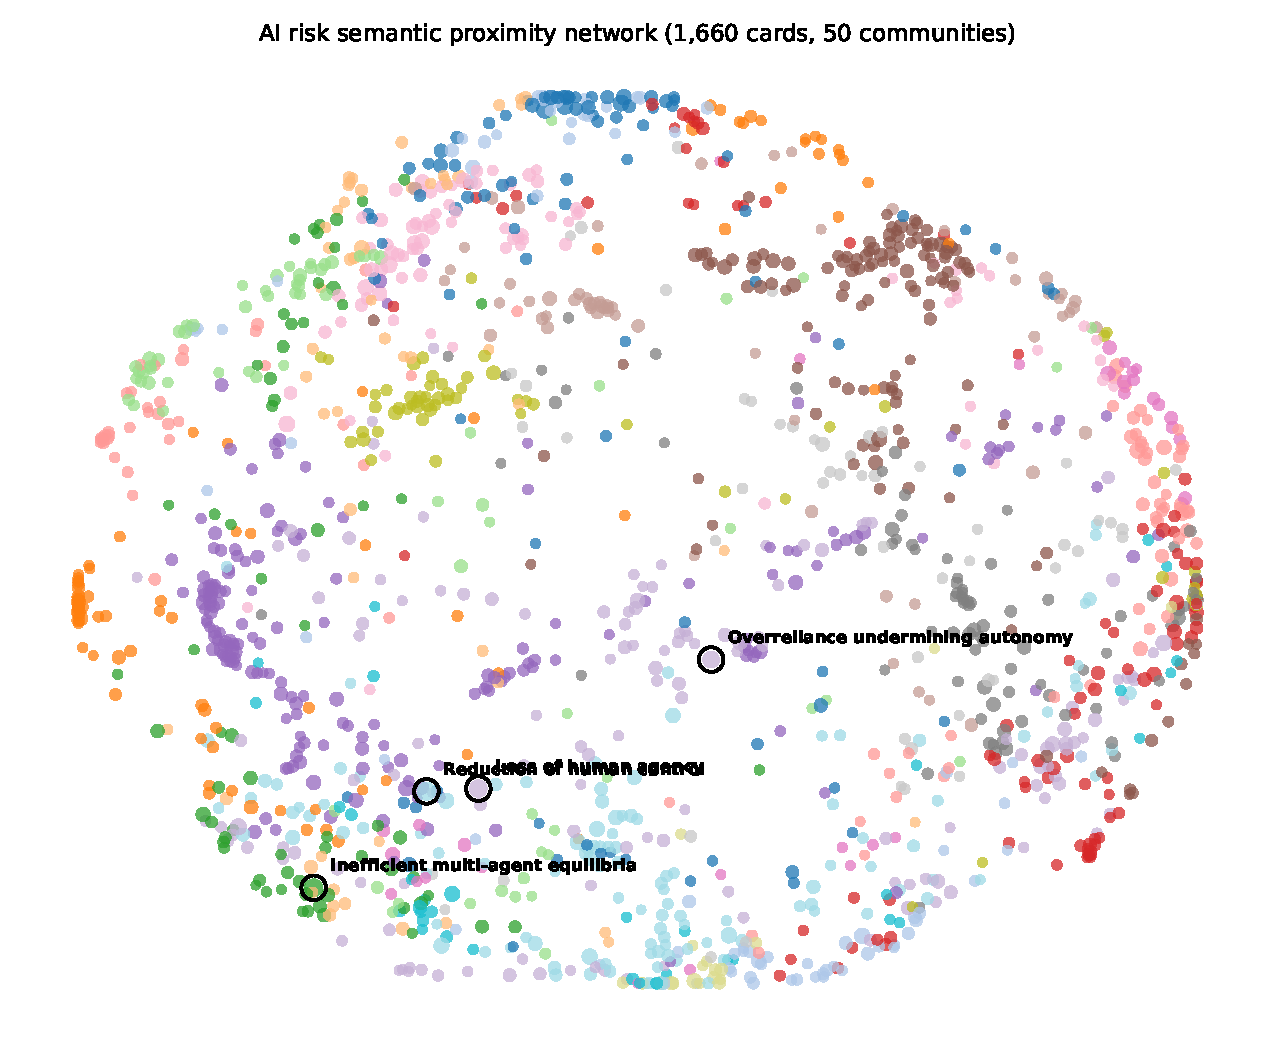
\includegraphics[width=0.95\linewidth]{fig1_semantic_space.pdf}
\caption{\textbf{The AI risk semantic proximity network.} 1,660 active risk cards (v2.17.2), positioned by force-directed layout, colored by their dominant community (50 communities from graph-regularized seeded spherical EM), and sized by degree. Circled nodes mark the four loss-of-control hubs discussed in the text.}
\label{fig:space}
\end{figure}

\subsection*{Overlapping communities quantify what trees discard}

The graph-regularized seeded spherical EM converges to 50 communities ranging in size from 2 to 140 cards (median 25). The largest communities concern weaponization (140 cards), policy exposure (114), non-contestability (90), anthropomorphism (71), and misinformation and disinformation (68). Community affiliation is computed as a profile rather than a single label: a card is affiliated with every community in which its affiliation weight exceeds a threshold of 0.03. Under this criterion, 459 cards (27.7\%) hold two or more community affiliations, with a maximum of eight. To our knowledge this is the first direct quantification, for an operational AI risk taxonomy, of how much relational information a single-parent hierarchy discards: more than a quarter of the catalog participates in conceptual neighborhoods that the published tree cannot express.

\subsection*{Hubs are semantic attractors, not statistical outliers}

The network is built by a union of $k$-nearest-neighbor relations, which imposes a degree floor near $k=10$ and deliberately suppresses extreme hubs; we therefore make no heavy-tailed or scale-free claims about the degree distribution, consistent with the methodological cautions of the power-law literature~\cite{clauset2009,broido2019}. What the construction does make interpretable is degree above the floor: a card's excess degree counts how many other cards selected it as one of their nearest semantic neighbors. High-degree nodes are thus semantic attractors, concepts that many specific risks find themselves close to.

Read this way, the top of the degree ranking is strikingly coherent (Fig.~\ref{fig:degree}a). The four highest-degree cards are: future AI systems actively reducing human control (degree 41, chosen as nearest neighbor by roughly 31 cards, three times the median); collectively inefficient equilibria among interacting AI agents (40); loss of human agency and autonomy (38); and overreliance on AI systems undermining user autonomy (34, tied). We refer to these as the loss-of-control constellation. Inequality across the network is otherwise modest (degree Gini 0.153, strength Gini 0.172, with only 2.1\% of nodes exceeding twice the median degree), which sharpens rather than dilutes the finding: the space has few privileged concepts, and those few are about control.

\begin{figure}[htbp]
\centering
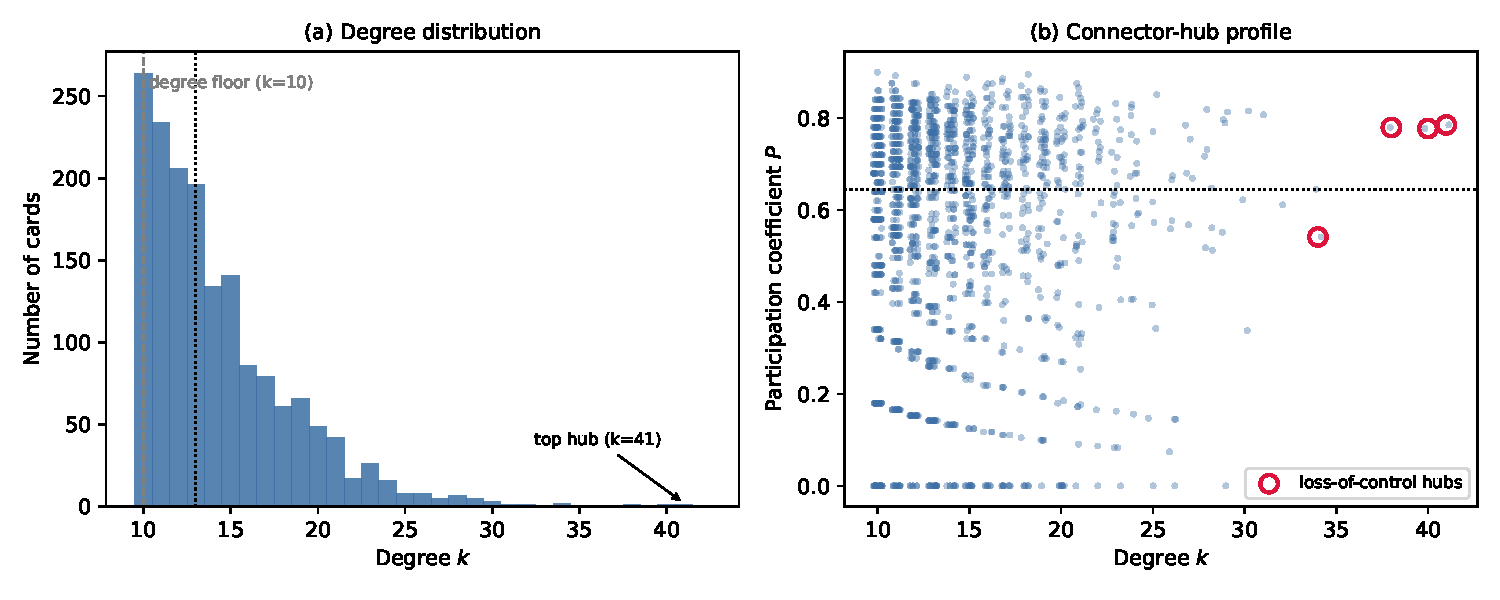
\includegraphics[width=\linewidth]{fig2_degree_participation.pdf}
\caption{\textbf{Degree structure and connector hubs.} (a) Degree distribution of the proximity network. The union-$k$NN construction imposes a floor near $k=10$ and suppresses hubs, so no heavy-tail claim is made; degree above the floor counts how often a card is chosen as a nearest neighbor. (b) Participation coefficient versus degree. The loss-of-control hubs (circled) combine high degree with high participation, marking them as connectors whose neighborhoods span up to ten communities.}
\label{fig:degree}
\end{figure}

\subsection*{The constellation bridges communities}

Degree alone cannot distinguish a concept that is central within one dense topic from one that connects the space. The participation coefficient~\cite{guimera2005} separates the two: the network-wide median is 0.645, and three of the four constellation hubs reach 0.78 to 0.79, with neighbors distributed across nine to ten of the fifty communities (Fig.~\ref{fig:degree}b). Reduction of human control, in particular, combines the highest degree in the network with a participation percentile of 84. These are connector hubs in the sense of Guimer\`a and Amaral: removing them would not disconnect the network, but it would remove the shortest conceptual paths between otherwise distant risk domains.

A curation signal corroborates the picture. Cards flagged HOLD, meaning that expert review has not yet finalized their placement, constitute 46.1\% of the catalog (765 cards), but 52.3\% of the top degree decile versus 45.3\% of the remainder. The concepts that are hardest to file under a single parent are disproportionately the ones the space treats as central, which is precisely what overlapping affiliation predicts.

\section*{Discussion}

Why do loss-of-control concepts occupy the center of the space? Three mutually consistent explanations emerge, and none reduces to curatorial bias. First, semantic generality: these are system-level concepts, and a very large number of concrete risks, from prompt-injected robots to manipulative recommender systems, are naturally phrased as specific ways of eroding human control, so their embeddings sit near many neighborhoods at once. Second, bridging position: the constellation's high participation coefficients show that it supplies the conceptual paths between communities as different as weaponization, anthropomorphism, and policy exposure; centrality here is a structural role, not a frequency effect. Third, theoretical consistency: an independent line of argument in the alignment literature, from the assurance problems of Russell~\cite{russell2019} through the extreme-risk analyses of Bengio and colleagues~\cite{bengio2024} to the gradual disempowerment thesis~\cite{kulveit2025}, predicts on first principles that control erosion is the common pathway through which heterogeneous AI harms compound. The semantic space, built with no knowledge of this literature, recovers its central claim as a topological fact.

Two reservations bound the interpretation. Semantic proximity is not causal transmission; an edge means two risks are described similarly, not that one triggers the other, and inferring propagation dynamics would require the interaction-network methods of systemic-risk research~\cite{helbing2013}. And the elevated HOLD share among hubs is not a defect of the taxonomy: it is the expected behavior of single-parent curation confronted with genuinely multi-community concepts, and it converts the semantic space into a practical instrument, since the space tells reviewers exactly which placements deserve their attention first.

For governance, the results argue that risk taxonomies should ship with their semantic space. The tree remains the administrative interface, but the space carries the information the tree discards: which risks are conceptual neighbors across branches, which concepts connect domains, and where single-parent placement is under strain. Because the entire pipeline, from document evidence to network, is versioned and recomputable, the space can be re-derived at every release and its topology tracked over time, turning claims about the changing structure of AI risk into measurements.

\section*{Methods}

\subsection*{Corpus provenance and card set}

The taxonomy's evidence chain is fully versioned: 3,906,767 collected documents were filtered to 82,971 AI-risk records, from which 1,726 candidate level-4 risk cards were generated; canonicalization reduced these to 1,711 cards, of which 1,660 are active in release v2.17.2 and analyzed here. Each card carries bilingual (Korean and English) labels and definitions. Expert-assigned severity, probability, and impact fields exist in the release but are excluded from all analyses in this paper. Card text (concatenated bilingual label and definition) is embedded with the BGE-M3 multilingual encoder~\cite{chen2024} under a pinned local snapshot with $L_2$ normalization, so inner products equal cosine similarities.

\subsection*{Constrained-EM placement audit}

Card placements are maintained by a guarded constrained-EM audit rather than unconstrained nearest-centroid assignment. For card $i$ and family $k$ the audit computes a composite score
\begin{equation}
S(i,k)=0.60\,c(i,k)+0.30\,d(i,k)+0.10\,w(i,k),
\end{equation}
combining centroid cosine similarity $c$, definition-level similarity $d$, and keyword similarity $w$. A placement moves only if the composite improvement is at least $0.020$ and the keyword-cosine gain is at least $0.015$; otherwise the incumbent placement is retained. The guards make the audit conservative by construction: it corrects clear misplacements while leaving debatable placements to expert review.

\subsection*{Graph-regularized seeded spherical EM}

Community structure is produced by a seeded spherical EM regularized on the proximity graph. The unregularized step alternates nearest-centroid assignment and normalized centroid recomputation,
\begin{equation}
z_i^{(t+1)}=\arg\max_k\; y_i^{\top}\mu_k^{(t)},\qquad
\mu_k^{(t+1)}=\frac{\sum_{i:z_i=k}y_i}{\lVert\sum_{i:z_i=k}y_i\rVert_2},
\end{equation}
where $y_i$ is the card embedding and $\mu_k$ the family centroid. The regularized objective adds a graph smoothness term with inverse temperature $\beta=18$ and coupling $\lambda=2$, and seed definitions enter with weight 5. The procedure converges in 16 iterations to a mean within-community similarity of 0.751 and defines the 50 communities used throughout. Affiliation weights below 0.03 are truncated; a card's community profile consists of all surviving affiliations.

\subsection*{Proximity network construction}

The base graph is a union of $k$-nearest-neighbor relations with $k=8$ and minimum cosine similarity 0.62, augmented by a projected neighborhood with $k=10$. Edge weights combine community-profile similarity and direct embedding similarity as $0.65\,s_{\mathrm{profile}}+0.35\,s_{\mathrm{direct}}$. Because every node contributes its own $k$ nearest neighbors, the construction imposes a degree floor near 10 and bounds hub formation; degree above the floor therefore counts incoming nearest-neighbor selections. Layout uses ForceAtlas2~\cite{jacomy2014} with fixed seed 42. All network statistics (density, clustering, assortativity, Gini coefficients, participation coefficients~\cite{guimera2005}) were computed directly from the released edge list and are exactly reproducible from the public data.

\subsection*{Exclusions and robustness stance}

No heavy-tailed or scale-free fits are attempted, because the union-$k$NN construction violates the sampling assumptions such fits require~\cite{clauset2009,broido2019}. All reported quantities are deterministic functions of the released v2.17.2 data with fixed seeds, and the analysis scripts reproduce every number in this paper from the public release.

\section*{Data availability}

All data are public and versioned. The taxonomy repository is at \url{https://github.com/deep1003/RAI-Risk-Taxonomy-2.0}; the analyzed release (v2.17.2) provides the proximity network (\texttt{semantic\_proximity\_network.json}) and card coordinates (\texttt{risk\_space.json}), and an interactive explorer is available at \url{https://deep1003.github.io/RAI-Risk-Taxonomy-2.0/risk-taxonomy-space.html}. An archived, DOI-minted copy of the release will be deposited on Zenodo upon acceptance.

\section*{Code availability}

The network construction and analysis scripts, including figure generation, are distributed with the repository and reproduce all statistics and figures in this paper from the public release.

\section*{Acknowledgements}
This work was supported by KT Corporation.

\section*{Author contributions}
Y.C. designed the study, performed the analyses, and wrote the manuscript. J.Y., Y.P., S.K., and J.C. contributed to the construction and expert review of the risk taxonomy and reviewed the manuscript. All authors approved the final version.

\section*{Competing interests}
The authors are employed by KT Corporation and declare no other competing interests.

\begin{thebibliography}{9}
\bibitem{slattery2024} Slattery, P., et al. The AI Risk Repository: A comprehensive meta-review, database, and taxonomy of risks from artificial intelligence. arXiv:2408.12622 (2024). \url{https://doi.org/10.48550/arXiv.2408.12622}.
\bibitem{chen2024} Chen, J., Xiao, S., Zhang, P., Luo, K., Lian, D. \& Liu, Z. M3-Embedding: Multi-linguality, multi-functionality, multi-granularity text embeddings through self-knowledge distillation. Findings of ACL 2024. \url{https://doi.org/10.18653/v1/2024.findings-acl.137}.
\bibitem{clauset2009} Clauset, A., Shalizi, C. R. \& Newman, M. E. J. Power-law distributions in empirical data. SIAM Rev. 51, 661--703 (2009). \url{https://doi.org/10.1137/070710111}.
\bibitem{broido2019} Broido, A. D. \& Clauset, A. Scale-free networks are rare. Nat. Commun. 10, 1017 (2019). \url{https://doi.org/10.1038/s41467-019-08746-5}.
\bibitem{guimera2005} Guimer\`a, R. \& Amaral, L. A. N. Functional cartography of complex metabolic networks. Nature 433, 895--900 (2005). \url{https://doi.org/10.1038/nature03288}.
\bibitem{russell2019} Russell, S. Human Compatible: Artificial Intelligence and the Problem of Control (Viking, 2019).
\bibitem{bengio2024} Bengio, Y., et al. Managing extreme AI risks amid rapid progress. Science 384, 842--845 (2024). \url{https://doi.org/10.1126/science.adn0117}.
\bibitem{kulveit2025} Kulveit, J., et al. Gradual disempowerment: Systemic existential risks from incremental AI development. arXiv:2501.16946 (2025). \url{https://doi.org/10.48550/arXiv.2501.16946}.
\bibitem{helbing2013} Helbing, D. Globally networked risks and how to respond. Nature 497, 51--59 (2013). \url{https://doi.org/10.1038/nature12047}.
\bibitem{jacomy2014} Jacomy, M., Venturini, T., Heymann, S. \& Bastian, M. ForceAtlas2, a continuous graph layout algorithm for handy network visualization designed for the Gephi software. PLoS ONE 9, e98679 (2014). \url{https://doi.org/10.1371/journal.pone.0098679}.
\end{thebibliography}

\end{document}
